% !TeX document-id = {a90a2b0a-e08e-44ed-850a-35793bedbf3a}
% !TeX TS-program = xelatex

% !BIB program = biber
\documentclass[handout]{beamer}
%\documentclass[compress]{beamer}
\usepackage[T1]{fontenc}
\usepackage{pifont}
\usetheme[block=fill,subsectionpage=progressbar,sectionpage=progressbar]{metropolis} 


\definecolor{Purple}{HTML}{911146}
\definecolor{Orange}{HTML}{CF4A30}

% Theme colors are derived from these two elements
\setbeamercolor{alerted text}{fg=Orange}

% ... however you can of course override styles of all elements
\setbeamercolor{frametitle}{bg=Purple}


\usepackage{wasysym}
\usepackage{etoolbox}
\usepackage[utf8]{inputenc}

\usepackage{threeparttable}
\usepackage{subcaption}

\usepackage{tikz-qtree}
\setbeamercovered{still covered={\opaqueness<1->{5}},again covered={\opaqueness<1->{100}}}


\usepackage{listings}

\lstset{
	basicstyle=\scriptsize\ttfamily,
	columns=flexible,
	breaklines=true,
	numbers=left,
	%stepsize=1,
	numberstyle=\tiny,
	backgroundcolor=\color[rgb]{0.85,0.90,1}
}



\lstnewenvironment{lstlistingoutput}{\lstset{basicstyle=\footnotesize\ttfamily,
		columns=flexible,
		breaklines=true,
		numbers=left,
		%stepsize=1,
		numberstyle=\tiny,
		backgroundcolor=\color[rgb]{.7,.7,.7}}}{}


\lstnewenvironment{lstlistingoutputtiny}{\lstset{basicstyle=\tiny\ttfamily,
		columns=flexible,
		breaklines=true,
		numbers=left,
		%stepsize=1,
		numberstyle=\tiny,
		backgroundcolor=\color[rgb]{.7,.7,.7}}}{}


\usepackage[american]{babel}
\usepackage{csquotes}
\usepackage[style=apa, backend = biber]{biblatex}
\DeclareLanguageMapping{american}{american-UoN}
\addbibresource{../literature.bib}
\renewcommand*{\bibfont}{\tiny}

\usepackage{tikz}
\usetikzlibrary{shapes,arrows,matrix}
\usepackage{multicol}

\usepackage{subcaption}

\usepackage{booktabs}
\usepackage{graphicx}

\graphicspath{{../pictures/}}

\makeatletter
\setbeamertemplate{headline}{%
	\begin{beamercolorbox}[colsep=1.5pt]{upper separation line head}
	\end{beamercolorbox}
	\begin{beamercolorbox}{section in head/foot}
		\vskip2pt\insertnavigation{\paperwidth}\vskip2pt
	\end{beamercolorbox}%
	\begin{beamercolorbox}[colsep=1.5pt]{lower separation line head}
	\end{beamercolorbox}
}
\makeatother



\setbeamercolor{section in head/foot}{fg=normal text.bg, bg=structure.fg}



\newcommand{\question}[1]{
	\begin{frame}[plain]
		\begin{columns}
			\column{.3\textwidth}
			\makebox[\columnwidth]{
				
\includegraphics[width=\columnwidth,height=\paperheight,keepaspectratio]{../pictures/mannetje.png}}
			\column{.7\textwidth}
			\large
			\textcolor{orange}{\textbf{\emph{#1}}}
		\end{columns}
\end{frame}}

\newcommand{\instruction}[1]{\emph{\textcolor{gray}{[#1]}}}


\title[Computational Communication Science 2]{\textbf{Computational Communication Science 2} \\Week 7 - Lecture\\ »Rule-based text classification and an introduction to supervised machine learning«}
\author[Marthe Möller, Anne Kroon]{Marthe Möller \\ Anne Kroon \\ ~ \\ \footnotesize{A.M.Moller@uva.nl, @MartheMoller \\a.c.kroon@uva.nl, @annekroon} \\}
\date{April, 2022}
\institute[Digital Society Minor, University of Amsterdam]{Digital Society Minor, University of Amsterdam}


\begin{document}
	
	\begin{frame}{}
		\titlepage
	\end{frame}
	
	\begin{frame}{Today}
		\tableofcontents
	\end{frame}

\begin{frame} 
	All course materials can be found at\ldots \\
	~~~~~~~~\url{https://github.com/annekroon/CCS-2}
\end{frame}

\section{Introducing\ldots}
\subsection{\ldots the people}

\begin{frame} 
	Introducing\ldots \\
	~~~~~~~~\ldots the people
\end{frame}


\begin{frame}{Introducing\ldots} {\huge{Marte}} \small{} 
	
	\begin{columns}
		\column{.3\textwidth}
		\makebox[\columnwidth]{
			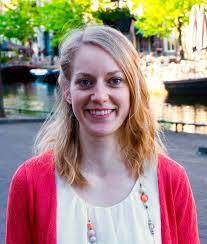
\includegraphics[width=\columnwidth,height=\paperheight,keepaspectratio]{../pictures/marthe.jpg}}
		\column{.7\textwidth}
		dr. Marthe Möller \\
		Assistant Professor
		\begin{itemize}
			\item interested in... 
		\end{itemize}
		@marthemoller \textbar A.M.Moller@uva.nl, \textbar \url{https://www.uva.nl/profiel/m/o/a.m.moller/a.m.moller.html} 
	\end{columns}
\end{frame}

\begin{frame}{Introducing\ldots} {\huge{Anne}} \small{} 
	\begin{columns}[] \column{.3\textwidth} \makebox[\columnwidth]{ 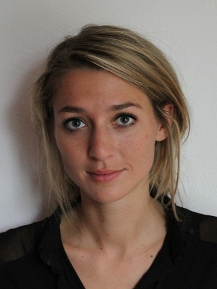
\includegraphics[width=\columnwidth,height=\paperheight,keepaspectratio]{../pictures/anne.jpg}} \column{.7\textwidth} dr. Anne Kroon \\ 
		Assistant Professor Corporate Communication
		\begin{itemize} 
			%\item Studied Journalism and Communication,  2006 - 2013
			%\item PhD candidate corporate communication at ASCoR (University of Amsterdam), 2014 - 2017
			\item Research focus on biased AI in recruitment, and media bias regarding minorities
			\item text analysis using automated approaches, word embeddings
		\end{itemize} @annekroon \textbar a.c.kroon@uva.nl  \textbar \url{http://www.uva.nl/profiel/k/r/a.c.kroon/a.c.kroon.html} 
	\end{columns} 
\end{frame}


\begin{frame}{Introducing\ldots}
	{\huge{You}}
	\small{}
	\begin{columns}
		\column{.3\textwidth}
		\makebox[\columnwidth]{
			
\includegraphics[width=\columnwidth,height=\paperheight,keepaspectratio]{../pictures/mannetje.png}}
		\column{.7\textwidth}
		Your name?\\
		Your background?\\
		Your reason to follow this course?\\
		Do you have a dataset you are working on?
	\end{columns}
\end{frame}

% example with a reference

\section{An example with a reference}
\begin{frame}{Why program your own tool?}
	\begin{block}{\textcite{Vis2013}}
		``{[}\ldots{]} these {[}commercial{]} tools are often unsuitable for academic purposes because of their cost, along with the problematic `black box' nature of many of these tools.''
	\end{block}
\end{frame}

% This prints the bibliography on the slide


\section{An example with some Python code\dots}

\begin{frame}[fragile]{A simple bottom-up approach}
\begin{lstlisting}
from collections import Counter
texts = ["I really really really love him, I do", "I hate him"]

for t in texts:
    print(Counter(t.split()).most_common(3))
\end{lstlisting}

\begin{lstlistingoutput}
[('really', 3), ('I', 2), ('love', 1)]
[('I', 1), ('hate', 1), ('him', 1)]
\end{lstlistingoutput}
\end{frame}



\begin{frame}
	\frametitle{References}
	\printbibliography
\end{frame}
	

\end{document}